\chapter{Practical Snapshot Isolation}
% \section{Natural Concurrency Control}
\section{Practical Snapshot Isolation}


\subsection{Key Observations and Motivations}
In this project, we are targeting distributed systems that 
are used for web applications. 
First, \cite{lu2023ncc} makes some key observations about transactions in web applications.

\begin{enumerate}
    \item Transactions in web applications are usually short. This means that the possibility that transactions interleave with each other and induce write-write or read-write conflict is small.
    \item Transactions in web applications are usually read-dominant. This means interleaving read requests  is fine.
    \item In usual network environments, transactions will arrive naturally in the order they submit.
\end{enumerate}

By combining the observations, we can conclude that most transactions in web applications will naturally satisfy the snapshot isolation level.  However, existing snapshot isolation protocols take a pessimistic view of transaction conflicts. They use excessive locks, extra rounds of messages, etc. to ensure that transactions satisfy the snapshot isolation level even if they satisfy that naturally. Instead, we take a practical view of snapshot isolation. We have already observed that most transactions in web applications naturally satisfy snapshot isolations. We abort those transactions that do not satisfy snapshot isolation properties or violate committed transactions' read visibility. Our design is heavily inspired by \cite{lu2023ncc}.


\subsection{Overall Architecture}
\begin{figure}[H]
    \centering
    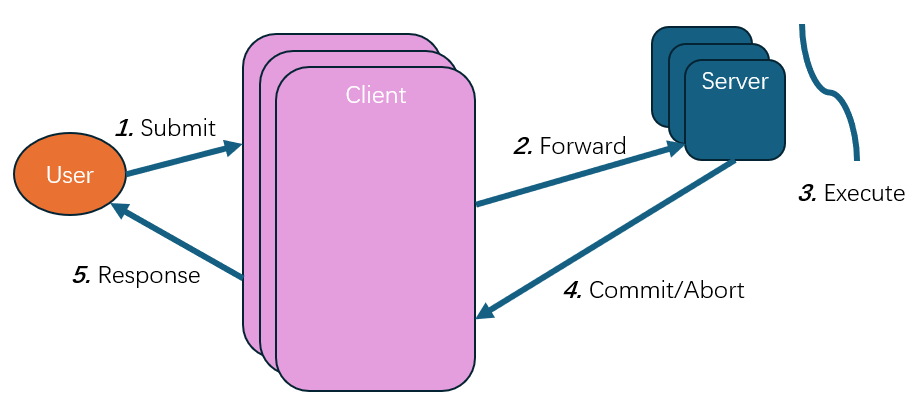
\includegraphics[width=0.8\linewidth]{figure/overall.png}
    \caption{Overall Architecture of Our Proposed Methods}
    \label{fig:overall}
\end{figure}

Figure \ref{fig:overall} describes our proposed methods' architecture. There are many clients and servers for scalability reasons. Each server holds one partition of the data. In the first step, users submit a transaction request to a client. In the second step, the client will look at the requests inside the transaction and forward the request to the server based on the request content (such as the hash value of the key involved in the transaction). The client will also assign a timestamp (such as a physical clock) to the transaction. In the third step, the server that receives the request will execute them in a non-blocking fashion, as we assume that most transactions will naturally satisfy the snapshot isolation property. After the execution finishes, the server will check whether the transaction satisfies the snapshot isolation properties. In rare cases where this transaction violates some properties, the server simply aborts it. In the fourth step, the server will send the decision on the commit/abort and the result to the client. In the fifth step, the client will return the result to the user.
\subsection{Non-blocking Execution}

The server will maintain the latest version tag for each data item it stores. 
The server executes the requests in a non-blocking manner. This means the server executes requests just as in a single thread. Moreover, when a read request is received, the server will execute the request and associate the result with its latest version. When a write request is received, the server will create a new version associated with that data item and associate that version with this write operation. This non-blocking execution greatly enhances the performance because it does not require blocking operations such as locking, extra rounds of messages.


\subsection{Server Side Algorithms}
Here we present our algorithms used at the server side. We adapt \cite{lu2023ncc} for snapshot isolation.


\begin{algorithm}
\caption{Server-side Algorithm for Executing Transactions of Practical Snapshot Isolation}
\label{alg:cap}
\begin{algorithmic}
\Require $S$ is a multi-version data store. $S[version][key]$ will retrieve the data item with key $key$ at the version $version$.
\Require $T$ is the transaction to be executed.
\Require $t$ is the latest system (or snapshot) version.
\Require $f(key)$ will return the largest version
of data item $key$ that is smaller than $t$. 
\Require $\mathcal{R}$ is the return result set.
\State $t^\prime \gets$  $t$ \Comment{Remember the system version before the transaction $T$}

\For{$r \in T$} \Comment{First, we execute all the requests in a non-blocking fashion.}
    \State $\mathcal{R}[r.key] \gets S[f(t^\prime)][r.key]$     \Comment{Retrieve the latest version result.}

\If {$r$ is a write request}
   % \State $\mathcal{R}[r.key] \gets S[t^\prime][r.key]$
    \State $t^\prime \gets t^\prime + 1$
    \State $S[t^\prime][r.key] \gets r.value$

\EndIf
\EndFor
\State $commit \gets true$
\Comment {Next, we will check whether to commit this transaction or not}
\For{$r \in T$}
\If {$r$ is a read request}
    \If {$t^\prime > f(r.key)$} \Comment{Read a future value, abort!}
    \State $commit \gets false$
    \EndIf
\Else \Comment{$r$ is a write request}
    \If {$t^\prime < f(r.key)$} \Comment{Overwrite a commit value, abort!}
    \State $commit \gets false$
    \EndIf
\EndIf
\EndFor


% \While{Server Does Not Receive a Request}
% \EndWhile
% \State $y \gets 1$
% \State $X \gets x$
% \State $N \gets n$
% \While{$N \neq 0$}
% \If{$N$ is even}
%     \State $X \gets X \times X$
%     \State $N \gets \frac{N}{2}$  
%     \Comment{This is a comment}
% \ElsIf{$N$ is odd}
%     \State $y \gets y \times X$
%     \State $N \gets N - 1$
% \EndIf
% \EndWhile
\end{algorithmic}
\end{algorithm}





\begin{algorithm}
\caption{The commit algorithm}\label{alg:commit}
\begin{algorithmic}
\Require $commit$ is $true$.
\Require $T$ the transaction to be executed
\State $t \gets t^\prime$ \Comment{Update the system version.}
\For {$r \in T$} \Comment{Update $f(key)$}
\If {$r$ is a write request}
\State $f(r.key) \gets t$
\EndIf
\EndFor
\end{algorithmic}
\end{algorithm}



\begin{algorithm}
\caption{The abort algorithm}\label{alg:abort}
\begin{algorithmic}
\Require $commit$ is $false$.
\Require $T$ the transaction to be aborted
\For {$r \in T$} 
% \Comment{Update $f(key)$}
\If {$r$ is a write request}
\State $S[f(r.key)][r.key] \gets \mathcal R[f(r.key)]$ \Comment{Rollback to the previous version}
\EndIf
\EndFor
\end{algorithmic}
\end{algorithm}


Algorithm \ref{alg:cap} is the main algorithm. Algorithm \ref{alg:commit} is the commit algorithm, and Algorithm \ref{alg:abort} is the abort algorithm. 
We use $S$ to record a multi-version data store, $t$ to record the latest system version, and $f(key)$ to retrieve the latest version of data item $key$. The algorithm first executes all requests in a non-blocking fashion. Then, it will check all requests and see if there are any read-write conflicts or write-write conflicts. If no such conflicts exist and the transaction can safely be committed, we update $t$ and $f(key)$ according to the commit algorithm. Otherwise, according to the abort algorithm, we will roll back $S$ to the previous version.  


\section{Experiments}
\subsection{Overview}
In this section, we will describe our experiments to demonstrate the performance of our practical snapshot isolation algorithm. We implemented three baselines. The first baseline we implemented is Clock-SI \cite{du2013clock}, a snapshot isolation algorithm that does not depend on a centralized clock. The second snapshot isolation algorithm we implemented is Percolator \cite{peng2010large}. Google widely uses the Percolator system to process incremental updates to a large data set. The Percolator system supports snapshot isolation protocol and provides an industrial common standard for implementing distributed snapshot isolation concurrency control levels. The third baseline we implemented is Walter \cite{sovran2011transactional}. It also supports (parallel) snapshot isolation. We will first introduce the three baselines. Then, we will introduce the experiment setup. Next, we will introduce and analyze the results of the experiment. Finally,  we will conclude this chapter. 


% \subsection{Clock-SI}



% \subsection{Percolator}
% \subsection{Walter}
\subsection{Experimental Setup}

\paragraph{Code Base.} We used the same code base as \cite{lu2023ncc} for implementing our practical snapshot isolation algorithms. We also used the same code base for implementing Clock-SI \cite{du2013clock}, Percolator \cite{peng2010large}, Walter \cite{sovran2011transactional}.

\paragraph{Workloads.} We used the YCSB benchmark \cite{cooper2010benchmarking}. YCSB is a key-value benchmark that Yahoo collects for many usages, including testing the performance of key-value stores, different concurrency control protocols. We mainly used workload A for testing. Workload A is a read-dominant workload, but the read-write ratio could be tuned for different purposes. Unless otherwise stated, we use the default parameter settings in YCSB.

\paragraph{Setup.} We used the CloudLab \cite{duplyakin2019design} as the testbed.  We used the XL170 node on the Utah cluster. The machine has 2 10-Core, 3.4 GHz, Xeon E5-2640 v4 CPUs and the network bandwidth is 10Gbps. 




\subsection{Results for Different Read Ratios}
We experiment with our methods with three other baselines under different read ratios. Refer to Figure \ref{fig:31}, Figure \ref{fig:32}, Figure \ref{fig:33}. Results show that our method outperforms three other baselines under different read ratio.

\begin{figure}[H]
    \centering
    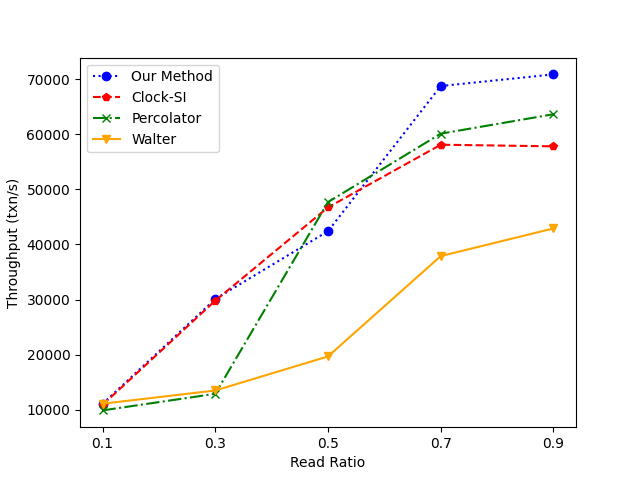
\includegraphics[width=0.8\linewidth]{figure/31.png}
    \caption{Throughput Comparison for Different Concurrency Control Algorithms for Different Read Ratio}
    \label{fig:31}
\end{figure}
\begin{figure}[H]
    \centering
    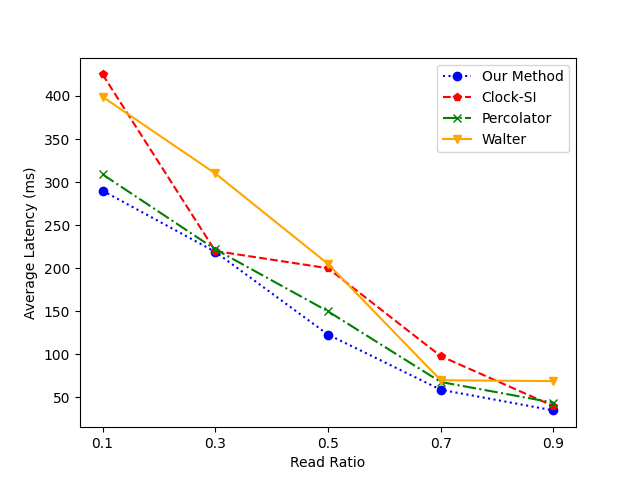
\includegraphics[width=0.8\linewidth]{figure/32.png}
    \caption{Average Latency for Different Concurrency Control Algorithms for Different Read Ratio}
    \label{fig:32}
\end{figure}
\begin{figure}[H]
    \centering
    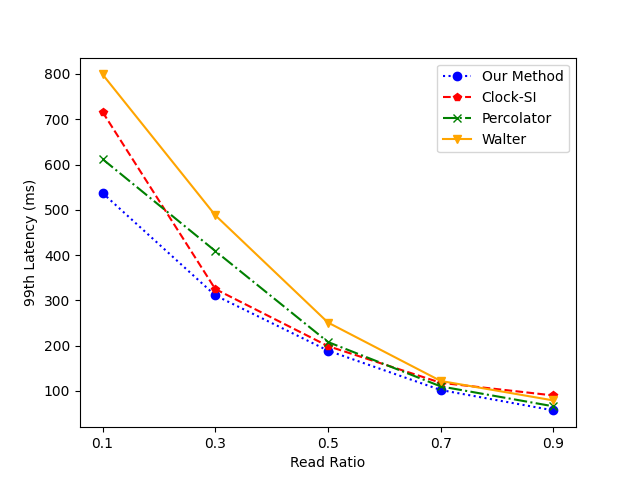
\includegraphics[width=0.8\linewidth]{figure/33.png}
    \caption{99th Latency for Different Concurrency Control Algorithms for Different Read Ratio}
    \label{fig:33}
\end{figure}



\subsection{Results for Different Transaction Sizes}
We experiment with our methods with three other baselines under different transaction sizes. Refer to Figure \ref{fig:34}, Figure \ref{fig:35}, Figure \ref{fig:36}. Results show that our method outperforms three other baselines under different transaction size.

\begin{figure}[H]
    \centering
    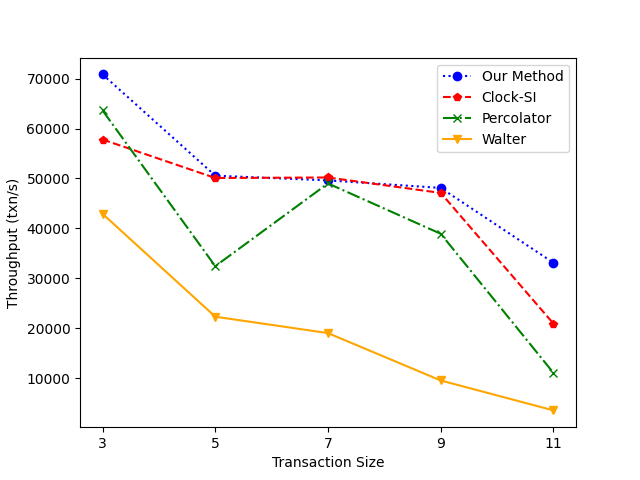
\includegraphics[width=0.8\linewidth]{figure/34.png}
    \caption{Throughput Comparison for Different Concurrency Control Algorithms for Different Transaction Size}
    \label{fig:34}
\end{figure}
\begin{figure}[H]
    \centering
    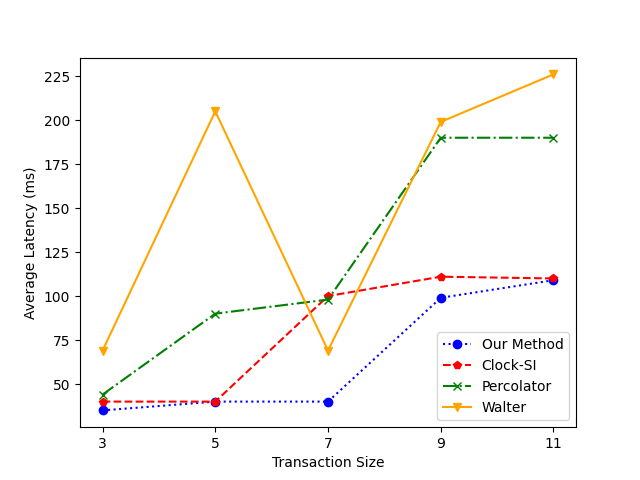
\includegraphics[width=0.8\linewidth]{figure/35.png}
    \caption{Average Latency for Different Concurrency Control Algorithms for Different Transaction Size}
    \label{fig:35}
\end{figure}
\begin{figure}[H]
    \centering
    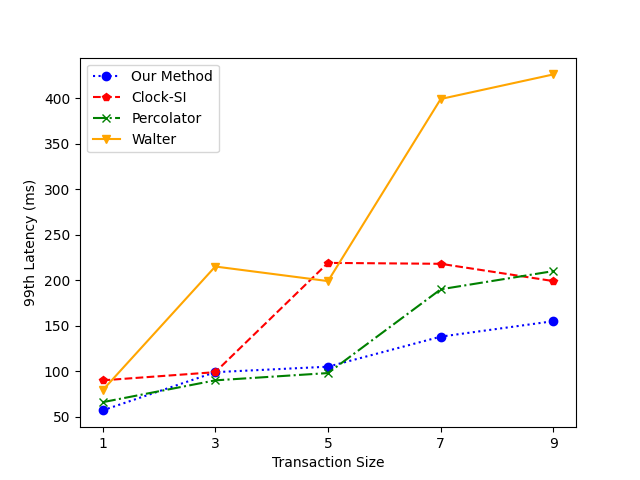
\includegraphics[width=0.8\linewidth]{figure/36.png}
    \caption{99th Latency for Different Concurrency Control Algorithms for Different Transaction Size}
    \label{fig:36}
\end{figure}








\subsection{Results for Different Numbers of Servers}

We experiment with our methods with three other baselines under different number of servers. Refer to Figure \ref{fig:37}, Figure \ref{fig:38}, Figure \ref{fig:39}. Results show that our method outperforms three other baselines under different number of servers.

\begin{figure}[H]
    \centering
    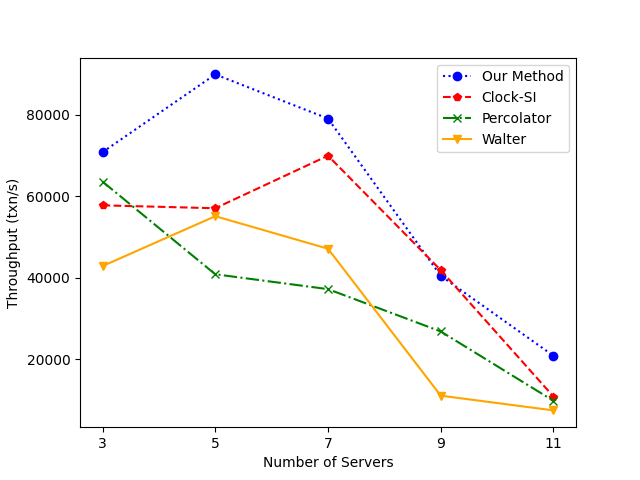
\includegraphics[width=0.8\linewidth]{figure/37.png}
    \caption{Throughput Comparison for Different Concurrency Control Algorithms for Different Number of Servers}
    \label{fig:37}
\end{figure}
\begin{figure}[H]
    \centering
    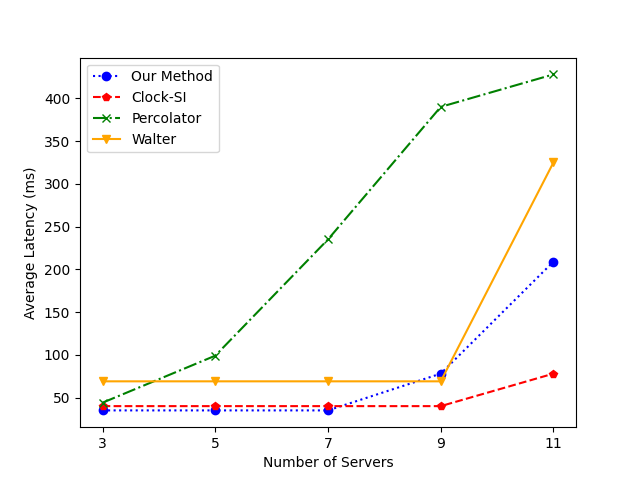
\includegraphics[width=0.8\linewidth]{figure/38.png}
    \caption{Average Latency for Different Concurrency Control Algorithms for Different Number of Servers}
    \label{fig:38}
\end{figure}
\begin{figure}[H]
    \centering
    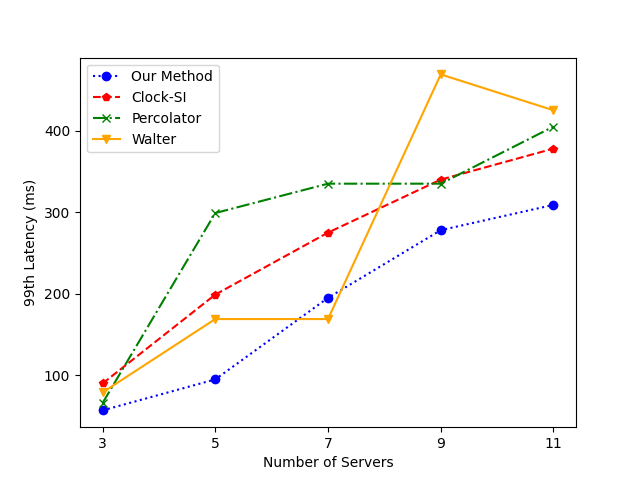
\includegraphics[width=0.8\linewidth]{figure/39.png}
    \caption{99th Latency for Different Concurrency Control Algorithms for Different Number of Servers}
    \label{fig:39}
\end{figure}



\subsection{Results for Different Numbers of Clients}
We experiment with our methods with three other baselines under different number of clients. Refer to Figure \ref{fig:40}, Figure \ref{fig:41}, Figure \ref{fig:42}. Results show that our method outperforms three other baselines under different number of clients.

\begin{figure}[H]
    \centering
    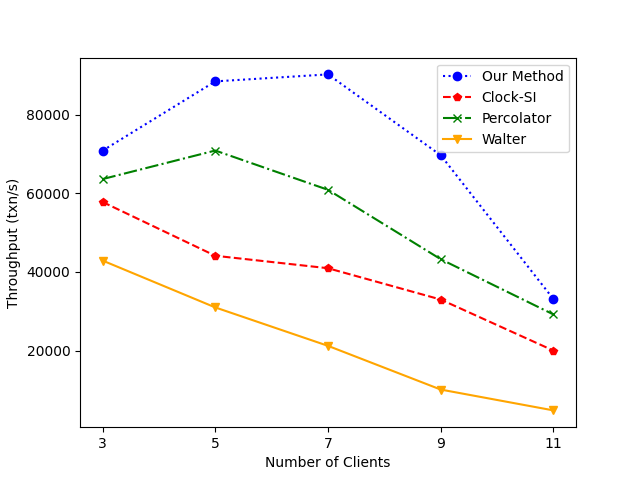
\includegraphics[width=0.8\linewidth]{figure/40.png}
    \caption{Throughput Comparison for Different Concurrency Control Algorithms for Different Number of Clients}
    \label{fig:40}
\end{figure}
\begin{figure}[H]
    \centering
    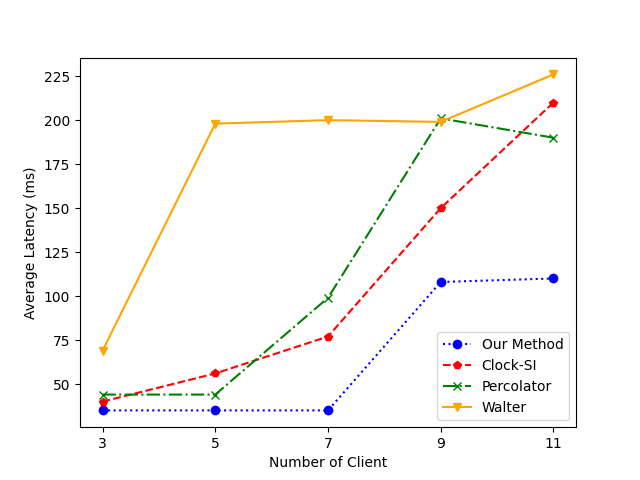
\includegraphics[width=0.8\linewidth]{figure/41.png}
    \caption{Average Latency for Different Concurrency Control Algorithms for Different Number of Client}
    \label{fig:41}
\end{figure}
\begin{figure}[H]
    \centering
    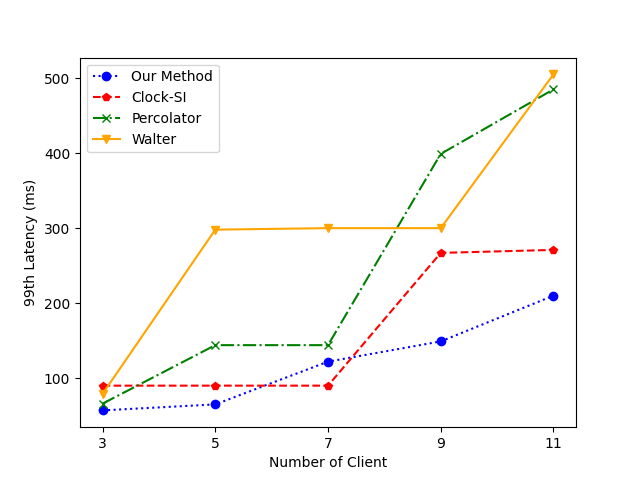
\includegraphics[width=0.8\linewidth]{figure/42.png}
    \caption{99th Latency for Different Concurrency Control Algorithms for Different Number of Clients}
    \label{fig:42}
\end{figure}



\subsection{Results for Different Value Sizes}
We experiment with our methods with three other baselines under different value size. Refer to Figure \ref{fig:43}, Figure \ref{fig:44}, Figure \ref{fig:45}. Results show that our method outperforms three other baselines under different value size.

\begin{figure}[H]
    \centering
    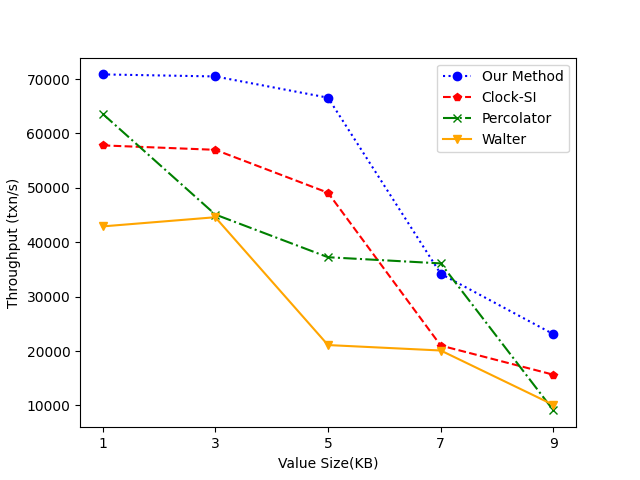
\includegraphics[width=0.8\linewidth]{figure/43.png}
    \caption{Throughput Comparison for Different Concurrency Control Algorithms for Different Value Size}
    \label{fig:43}
\end{figure}
\begin{figure}[H]
    \centering
    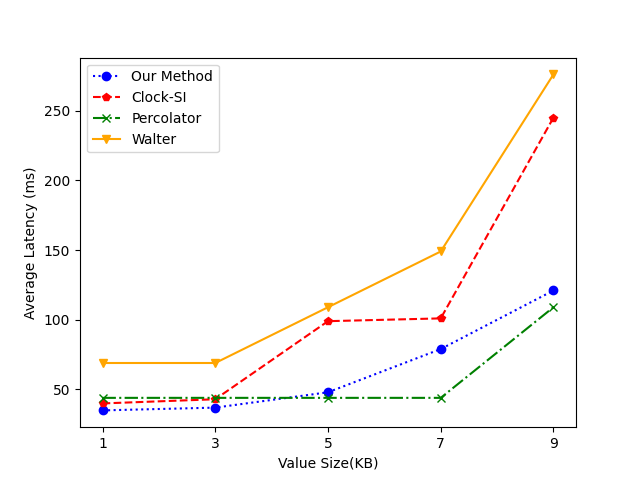
\includegraphics[width=0.8\linewidth]{figure/44.png}
    \caption{Average Latency for Different Concurrency Control Algorithms for Different Value Size}
    \label{fig:44}
\end{figure}
\begin{figure}[H]
    \centering
    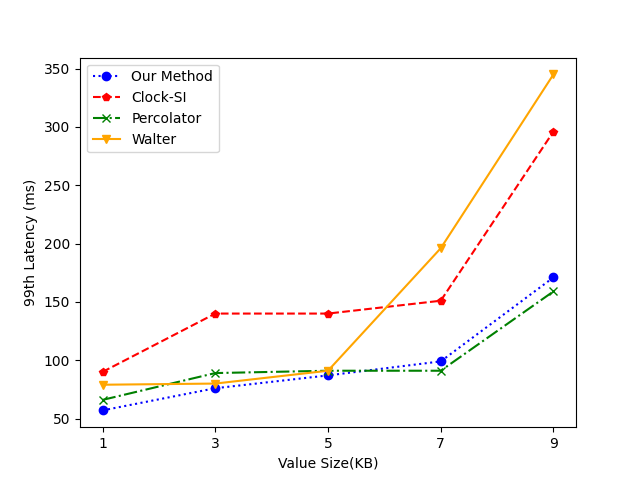
\includegraphics[width=0.8\linewidth]{figure/45.png}
    \caption{99th Latency for Different Concurrency Control Algorithms for Different Value Size}
    \label{fig:45}
\end{figure}




\subsection{Results for Different Numbers of Keys}

We experiment with our methods with three other baselines under different number of keys. Refer to Figure \ref{fig:46}, Figure \ref{fig:47}, Figure \ref{fig:48}. Results show that our method outperforms three other baselines under different number of keys.

\begin{figure}[H]
    \centering
    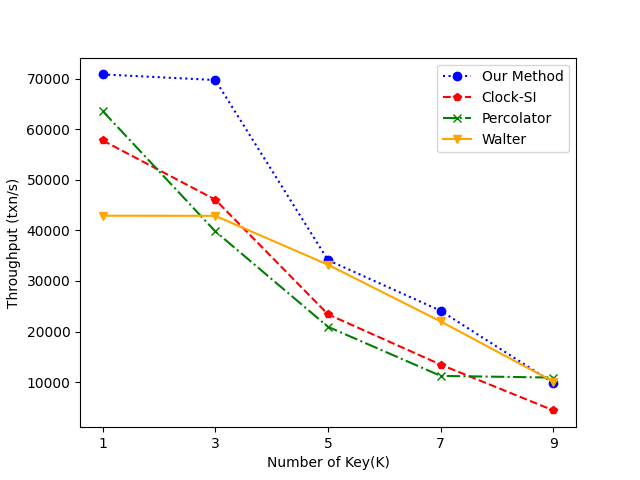
\includegraphics[width=0.8\linewidth]{figure/46.png}
    \caption{Throughput Comparison for Different Concurrency Control Algorithms for Different Number of Keys}
    \label{fig:46}
\end{figure}
\begin{figure}[H]
    \centering
    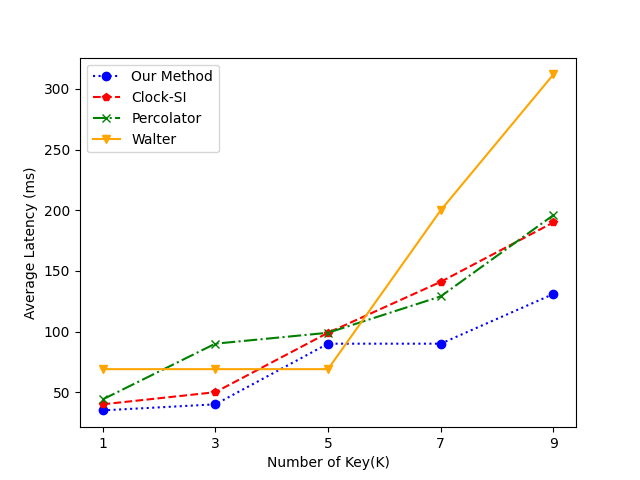
\includegraphics[width=0.8\linewidth]{figure/47.png}
    \caption{Average Latency for Different Concurrency Control Algorithms for Different Number of Keys}
    \label{fig:47}
\end{figure}
\begin{figure}[H]
    \centering
    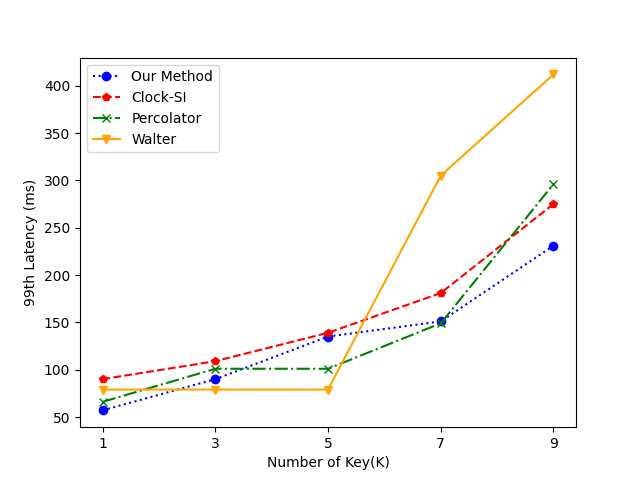
\includegraphics[width=0.8\linewidth]{figure/48.png}
    \caption{99th Latency for Different Concurrency Control Algorithms for Different Number of Keys}
    \label{fig:48}
\end{figure}




\subsection{Conclusions}
In this chapter, we have presented practical snapshot isolation algorithms based on the observation that most transactions will naturally be preserved in the order they submit by \cite{lu2023ncc}. As such, we take an optimistic approach. We execute the transaction without relying on external events such as lock. When the transaction is being committed, we will check whether the transaction satisfies the snapshot isolation properties. Our algorithms show  performance improvement over the three baselines implemented.
